
\section{树、标号与分割}\label{sec:D-2}

\emph{树}是没有圈的连通图。其顶点构成有限集 $T$，边构成关系
$E\subset T\times T$。（当 $\alpha E\beta$ 时，顶点 $\alpha$ 与 $\beta$
由一条边相连。）“没有圈的连通图”这一条件可表述为以下公理。

\noindent\textbf{（对称性）}若 $\alpha E\beta$，则 $\beta E\alpha$。

\noindent\textbf{（反自反性）}若 $\alpha E\beta$，则 $\alpha\ne\beta$。

\noindent\textbf{（连通性）}对任意 $\alpha,\beta\in T$ 且
$\alpha\ne\beta$，存在 $\gamma_0,\ldots,\gamma_m\in T$，满足
$\gamma_0=\alpha$、$\gamma_m=\beta$，且对所有 $i$ 有
$\gamma_iE\gamma_{i+1}$。

\noindent\textbf{（无圈性）}若 $\gamma_0,\ldots,\gamma_m\in T$，
对所有 $i$ 有 $\gamma_iE\gamma_{i+1}$、$\gamma_i\ne\gamma_{i+2}$，
则 $\gamma_0\ne\gamma_m$。

映射 $f:(T,E)\to(\widetilde T,\widetilde E)$ 称为\emph{\BookRecordIndex{T0305}树同态}，
若对所有 $\widetilde\alpha\in\widetilde T$，$f^{-1}(\widetilde\alpha)$
是一棵树，并且 $\alpha E\beta$ 蕴含
$f(\alpha)=f(\beta)$ 或 $f(\alpha)\widetilde E f(\beta)$。
若 $f$ 是双射，且 $f$ 与 $f^{-1}$ 都是\BookRecordIndex{T0305}树同态，则称为\emph{\BookRecordIndex{T0304}树同构}。
几何上，可把\BookRecordIndex{T0305}树同态看作将边压缩的映射。

设 $(T,E)$ 为树。对每对 $\alpha,\beta\in T$，存在唯一的有序顶点列
$\gamma_0,\ldots,\gamma_m\in T$（$m\ge0$），满足
\[
  \gamma_iE\gamma_{i+1},\qquad \gamma_i\ne\gamma_{i+2},\qquad
  \gamma_0=\alpha,\qquad\gamma_m=\beta.
\]
它称为从 $\alpha$ 到 $\beta$ 的\emph{（边）链}，链上的顶点集记作
\[
  [\alpha,\beta]:=[\beta,\alpha]:=\{\gamma_i\mid i=0,\ldots,m\}.
\]

\begin{figure}[tbp]
\centering
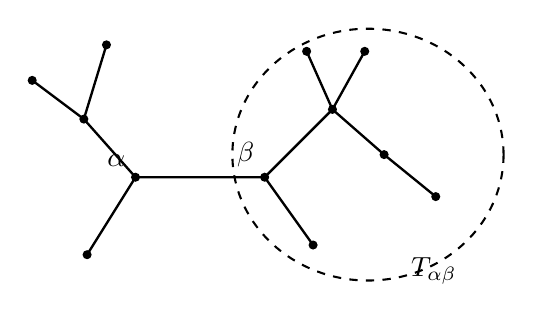
\begin{tikzpicture}[scale=.82,line width=.85pt]
  \coordinate (a) at (-.6,0);
  \coordinate (b) at (1.4,0);
  \coordinate (l) at (-1.4,.9);
  \coordinate (r) at (2.45,1.05);
  \coordinate (m) at (3.25,.35);
  \draw (a)--(b) (a)--(l) (a)--(-1.35,-1.2)
    (l)--(-2.2,1.5) (l)--(-1.05,2.05)
    (b)--(r) (b)--(2.15,-1.05)
    (r)--(2.05,1.95) (r)--(2.95,1.95) (r)--(m)
    (m)--(4.05,-.3);
  \draw[dashed,line width=.75pt] (3,.35) ellipse[x radius=2.1,y radius=1.95];
  \foreach \p in {a,b,l,r,m} \fill (\p) circle (2pt);
  \fill (-1.35,-1.2) circle (2pt);
  \fill (-2.2,1.5) circle (2pt);
  \fill (-1.05,2.05) circle (2pt);
  \fill (2.15,-1.05) circle (2pt);
  \fill (2.05,1.95) circle (2pt);
  \fill (2.95,1.95) circle (2pt);
  \fill (4.05,-.3) circle (2pt);
  \node[above left] at (a) {$\alpha$};
  \node[above left] at (b) {$\beta$};
  \node at (4.02,-1.45) {$T_{\alpha\beta}$};
\end{tikzpicture}

\caption{树。}\label{fig:D-2-1}
\end{figure}

特别地，$[\alpha,\alpha]=\{\alpha\}$。切断（即移除）任意一条边
$\alpha E\beta$，会把树 $T$ 分成两个连通分支。含 $\beta$ 的分支记为
$T_{\alpha\beta}$（见图~\ref{fig:D-2-1}）。它是从 $\alpha$
出发、经过 $\beta$ 的\BookRecordIndex{T0064}边链所能到达的所有顶点的集合。换言之，
\[
  T_{\alpha\beta}:=\{\gamma\in T\mid\beta\in[\alpha,\gamma]\}.
\]
此集合称为树 $T$ 的一个\emph{分支}。每条边 $\alpha E\beta$ 都把
$T$ 分解为分支 $T_{\alpha\beta}$ 与 $T_{\beta\alpha}$ 的不交并。

我们强调，树 $T$ 的边被视为无向的。因而可将边集与满足
$\alpha E\beta$ 的二元子集 $\{\alpha,\beta\}\subset T$ 组成的集合等同。
边数记为
\[
  e(T):=\#\{\text{边}\}=\#\{\text{顶点}\}-1.
\]
与此相对，$(\alpha,\beta)\in E$ 是有向边，其数目为
$2e(T)=\#E$。

\begin{exercise}\label{ex:D-2-1}
设 $(T,E)$ 与 $(\widetilde T,\widetilde E)$ 为树。证明：
$f:T\to\widetilde T$ 是\BookRecordIndex{T0305}树同态，当且仅当对所有 $\alpha,\beta\in T$ 有
$f([\alpha,\beta])=[f(\alpha),f(\beta)]$。
\end{exercise}

\begin{exercise}\label{ex:D-2-2}
设 $f:T\to\widetilde T$ 是满射\BookRecordIndex{T0305}树同态。证明：对
$\widetilde T$ 中的每条边 $\widetilde\alpha\widetilde E\widetilde\beta$，
$T$ 中存在唯一一条边 $\alpha E\beta$，使
$f(\alpha)=\widetilde\alpha$、$f(\beta)=\widetilde\beta$。
\end{exercise}

\noindent\textbf{标号。}
固定整数 $n\ge3$。一个\emph{带 $n$ 个标号的树}是三元组
$(T,E,\Lambda)$，其中 $(T,E)$ 是树，且
$\Lambda=\{\Lambda_\alpha\}_{\alpha\in T}$ 将指标集
$\{1,\ldots,n\}$ 分解为不交并
\[
  \{1,\ldots,n\}=\bigsqcup_{\alpha\in T}\Lambda_\alpha.
\]
若对每个 $\alpha\in T$ 都有
\begin{equation}\label{eq:D-2-1}
  n_\alpha=\#\Lambda_\alpha
    +\#\{\beta\in T\mid\alpha E\beta\}\ge3,
\end{equation}
则称此标号\emph{稳定}。带稳定 $n$-标号的树称为\emph{稳定树}。
两棵带 $n$ 个标号的树 $(T,E,\Lambda)$ 与
$(\widetilde T,\widetilde E,\widetilde\Lambda)$ 称为\emph{同构}，
若存在\BookRecordIndex{T0304}树同构 $f:T\to\widetilde T$，使得对每个 $\alpha\in T$ 有
$\widetilde\Lambda_{f(\alpha)}=\Lambda_\alpha$。
稳定带 $n$ 个标号树的同构类集合记为 $\mathcal L_n$。\footnote{这里滥用了记号。
严格说来，带 $n$ 个标号的树构成范畴而非集合，因此它们的同构类不构成集合。
不过此处略去这一点，权且把这些同构类当作集合。下文定理~\ref{thm:D-2-6}
表明，实际上这样的同构类只有有限多个。若要使术语完全严格，可只考虑顶点属于
某个给定集合的树，但这里不这样做。}

\begin{lemma}\label{lem:D-2-3}
设 $(T,E,\Lambda)$ 为带 $n$ 个标号的树。则
\[
  \sum_{\alpha\in T}(n_\alpha-3)+e(T)=n-3.
\]
\end{lemma}
\begin{proof}
记 $E_\alpha:=\{\beta\in T\mid\alpha E\beta\}$。则对
$\alpha\in T$，有 $n_\alpha=\#\Lambda_\alpha+\#E_\alpha$，并且
$\sum_{\alpha\in T}\#E_\alpha=\#E=2e(T)$。因此
\[
  \sum_{\alpha\in T}(n_\alpha-3)
  =\sum_{\alpha\in T}\#\Lambda_\alpha
   +\sum_{\alpha\in T}\#E_\alpha-3(e(T)+1)
  =n-3-e(T).
\]
这证明了引理。
\end{proof}

树 $(T,E)$ 的 $n$-标号也可表为函数
\[
  \{1,\ldots,n\}\longrightarrow T:\quad i\longmapsto\alpha_i,
\]
其中 $\alpha_i=\alpha$ 当且仅当 $i\in\Lambda_\alpha$。
给定任意三个互异指标 $i,j,k\in\{1,\ldots,n\}$，记
$\alpha(i,j,k)\in T$ 为满足
\begin{equation}\label{eq:D-2-2}
  \{\alpha(i,j,k)\}
   =[\alpha_i,\alpha_j]\cap[\alpha_j,\alpha_k]
       \cap[\alpha_k,\alpha_i]
\end{equation}
的唯一顶点（见习题~\ref{ex:D-2-4} 及图~\ref{fig:D-2-2}）。
若 $\alpha_i,\alpha_j,\alpha_k$ 两两不同，则 $\alpha=\alpha(i,j,k)$
的特征是：$\alpha_i,\alpha_j,\alpha_k$ 分别位于分解
\[
  T=\{\alpha\}\cup\bigcup_{\beta\in T,\,\alpha E\beta}T_{\alpha\beta}
\]
中的三个不同集合。另一方面，若 $\alpha_i,\alpha_j,\alpha_k$
中至少两个等于 $\beta$，则 $\alpha(i,j,k)=\beta$。

\begin{figure}[tbp]
\centering
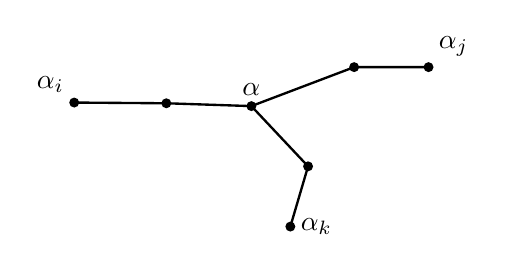
\begin{tikzpicture}[scale=.9,line width=.85pt]
  \coordinate (a) at (0,0);
  \coordinate (li) at (-2.5,.05);
  \coordinate (lj) at (2.5,.55);
  \coordinate (lk) at (.55,-1.7);
  \draw (a)--(-1.2,.04)--(li)
    (a)--(1.45,.55)--(lj)
    (a)--(.8,-.85)--(lk);
  \foreach \p in {a,li,lj,lk} \fill (\p) circle (2pt);
  \fill (-1.2,.04) circle (2pt);
  \fill (1.45,.55) circle (2pt);
  \fill (.8,-.85) circle (2pt);
  \node[above] at (a) {$\alpha$};
  \node[above left] at (li) {$\alpha_i$};
  \node[above right] at (lj) {$\alpha_j$};
  \node[right] at (lk) {$\alpha_k$};
\end{tikzpicture}

\caption{树三角形。}\label{fig:D-2-2}
\end{figure}

\begin{exercise}\label{ex:D-2-4}
设 $(T,E)$ 为树。证明：对任意三个顶点 $\alpha,\beta,\gamma$，
交集 $[\alpha,\beta]\cap[\beta,\gamma]\cap[\gamma,\alpha]$
恰由一个点组成。
\end{exercise}

\begin{exercise}\label{ex:D-2-5}
证明稳定性条件~\eqref{eq:D-2-1} 等价于：每个 $\alpha\in T$
都可写成 $\alpha=\alpha(i,j,k)$，其中 $i,j,k$ 是三个互异指标。
\end{exercise}

Manin 在~\srcite{286} 第 III 章 $\S2.1$ 中引入以下术语。
他把\BookRecordIndex{T0084}带标号树定义为四元组 $(F,V,\delta,j)$，其中 $F,V$ 是有限集，
$\delta:F\to V$ 是映射，$j:F\to F$ 是对合。$F$ 的元素称为\BookRecordIndex{T0274}旗，
$V$ 的元素称为顶点，$\delta$ 称为\BookRecordIndex{T0063}边界映射。$j$ 的不动点对应\BookRecordIndex{T0066}标记点，
二元轨道对应边。因此\BookRecordIndex{T0274}旗集既包含所有满足 $\alpha E\beta$ 的有序顶点对
$(\alpha,\beta)$，又包含指示\BookRecordIndex{T0066}标记点位置的另外 $n$ 个\BookRecordIndex{T0274}旗。
几何上，\BookRecordIndex{T0274}旗 $f\in F$ 可看作在端点处附着于顶点 $\delta(f)$ 的半开区间。

\noindent\textbf{分割。}
下面将借助由切断边所得的指标集二分，给出带 $n$ 个标号树的另一种描述。
这些二分组成某些偏序集；我们将证明，可由相关分割系恢复稳定树的同构类。

我们用不含最后一个指标 $n$ 的子集 $I$ 描述一个分割。具体说，子集
$I\subset\{1,\ldots,n\}$ 称为一个\emph{\BookRecordIndex{T0008}$n$-分割}，若
\[
  2\le\#I\le n-2,\qquad n\notin I.
\]
注意若 $I$ 是分割，则 $I$ 与 $\{1,\ldots,n\}\setminus I$ 都至少含两个元素。
下文将看到，这一条件对应于稳定性。全体 \BookRecordIndex{T0008}$n$-分割的集合记为
$\mathcal I_n$。一个\emph{\BookRecordIndex{T0008}$n$-分割网络}是分割集
$S\subset\mathcal I_n$，满足\BookRecordIndex{T0348}相容性条件
\begin{equation}\label{eq:D-2-3}
  I,J\in S,\ I\cap J\ne\varnothing
  \quad\Longrightarrow\quad I\subset J\text{ 或 }J\subset I.
\end{equation}
此条件表明，按包含关系排序时，$S$ 是一个偏序集，
其中每个元素至多有一个紧邻的上方元素，但可以有多个紧邻的下方元素。
所有 \BookRecordIndex{T0008}$n$-分割网络构成的集合记为 $\mathcal S_n$。
空网络 $S=\varnothing$ 也属于 $\mathcal S_n$。

现在设 $(T,E,\Lambda)$ 是稳定的带 $n$ 个标号树。一个
\emph{$(T,E,\Lambda)$-分割}是满足下述条件的 \BookRecordIndex{T0008}$n$-分割
$I\in\mathcal I_n$：
\begin{equation}\label{eq:D-2-4}
  i,i'\in I,\ j,j'\notin I
  \quad\Longrightarrow\quad
  [\alpha_i,\alpha_{i'}]\cap[\alpha_j,\alpha_{j'}]=\varnothing.
\end{equation}
下述定理表明，可把这种分割视为移除一条边后，把 $T$ 分成两个连通\BookRecordIndex{T0417}子树。
它还表明，这些分割的全体构成一个 \BookRecordIndex{T0008}$n$-分割网络，并建立稳定\BookRecordIndex{T0084}带标号树与
\BookRecordIndex{T0008}$n$-分割网络之间的一一对应。

\begin{theorem}\label{thm:D-2-6}
\textup{(i)} 对每棵稳定的带 $n$ 个标号树 $(T,E,\Lambda)$，
其 $(T,E,\Lambda)$-分割的集合
\[
  S(T,E,\Lambda):=\{I\in\mathcal I_n\mid\text{$I$ 满足~\eqref{eq:D-2-4}}\}
\]
是一个 \BookRecordIndex{T0008}$n$-分割网络。

\textup{(ii)} 设 $(T,E,\Lambda)$ 是稳定的带 $n$ 个标号树，
$I\subset\{1,\ldots,n\}$。则 $I\in S(T,E,\Lambda)$ 当且仅当
存在边 $\alpha E\beta$，使 $\alpha_n\in T_{\alpha\beta}$ 且
\[
  I=I_{\beta\alpha}(T,E,\Lambda):=
    \{i\in\{1,\ldots,n\}\mid\alpha_i\in T_{\beta\alpha}\}.
\]

\textup{(iii)} 映射
$\mathcal L_n\to\mathcal S_n:[T,E,\Lambda]\mapsto S(T,E,\Lambda)$
是双射。

\textup{(iv)} 设 $(T,E,\Lambda)$ 与
$(\widetilde T,\widetilde E,\widetilde\Lambda)$ 是稳定的带 $n$ 个标号树。
对 $i=1,\ldots,n$，以 $i\in\Lambda_{\alpha_i}\cap
\widetilde\Lambda_{\widetilde\alpha_i}$ 定义
$\alpha_i\in T$ 与 $\widetilde\alpha_i\in\widetilde T$。则
\[
  S(\widetilde T,\widetilde E,\widetilde\Lambda)
  \subset S(T,E,\Lambda)
\]
当且仅当存在\BookRecordIndex{T0305}树同态 $f:T\to\widetilde T$，使对所有 $i$ 有
$f(\alpha_i)=\widetilde\alpha_i$。若成立，此\BookRecordIndex{T0305}树同态必为满射，
且对所有 $i,j,k$ 有 $f(\alpha(i,j,k))=\widetilde\alpha(i,j,k)$。
\end{theorem}

\begin{proof}
先证 (i)。设 $(T,E,\Lambda)$ 为稳定的带 $n$ 个标号树。
反设 $S(T,E,\Lambda)$ 不是 \BookRecordIndex{T0008}$n$-分割网络。则存在
$I,J\in S(T,E,\Lambda)$，满足
$I\cap J\ne\varnothing$、$I\not\subset J$、$J\not\subset I$。
选取 $i\in I\setminus J$、$j\in J\setminus I$ 与
$\nu\in I\cap J$。由于 $\nu,i\in I$，且 $j,n\notin I$，有
$[\alpha_\nu,\alpha_i]\cap[\alpha_j,\alpha_n]=\varnothing$；
又由于 $\nu,j\in J$，且 $i,n\notin J$，有
$[\alpha_\nu,\alpha_j]\cap[\alpha_i,\alpha_n]=\varnothing$。
但两条件不可能同时成立。这证明了 (i)。

再证 (ii)。先设 $I=I_{\beta\alpha}(T,E,\Lambda)$，其中
$\alpha E\beta$ 且 $\alpha_n\in T_{\alpha\beta}$。
显然 $n\notin I$。由~\eqref{eq:D-2-1}，树的每个端点至少带两个标号。
由于每个分支 $T_{\alpha\beta}$ 都包含至少一个端点，
故 $2\le\#I\le n-2$。当 $i,i'\in I$ 时，
$[\alpha_i,\alpha_{i'}]\subset T_{\beta\alpha}$；当 $j,j'\notin I$ 时，
$[\alpha_j,\alpha_{j'}]\subset T_{\alpha\beta}$。
故 $I$ 满足~\eqref{eq:D-2-4}，于是 $I\in S(T,E,\Lambda)$。

反过来，设 $I\in S(T,E,\Lambda)$，并定义
\[
  T_I:=\{\alpha(i,j,k)\mid\#(\{i,j,k\}\cap I)\ge2\}
    \subset\bigcup_{i,i'\in I}[\alpha_i,\alpha_{i'}],
\]
\[
  T_J:=\{\alpha(i,j,k)\mid\#(\{i,j,k\}\cap I)\le1\}
    \subset\bigcup_{j,j'\notin I}[\alpha_j,\alpha_{j'}].
\]
由习题~\ref{ex:D-2-5}，$T_I\cup T_J=T$；由~\eqref{eq:D-2-4}，
$T_I\cap T_J=\varnothing$。因此，上述两个包含关系实际上都是等号。
于是容易检查 $T_I$ 与 $T_J$ 都是树。具体说，若
$\alpha,\alpha'\in T_I$，\sourcefootnote{原书此处写 $\alpha,\alpha'\in T$，
但这里要证明 $T_I$ 的连通性，且随后要求连接链落在 $T_I$；按紧前的
$T_I$ 定义，改为 $\alpha,\alpha'\in T_I$。}
则存在 $i,i'\in I$，使得
\[
  [\alpha_i,\alpha]\cup[\alpha,\alpha']\cup
  [\alpha',\alpha_{i'}]=[\alpha_i,\alpha_{i'}]\subset T_I.
\]
由于 $T_I,T_J$ 都是树，存在唯一的边 $\alpha E\beta$，
其中 $\alpha\in T_I$、$\beta\in T_J$。于是
$T_I=T_{\beta\alpha}$、$T_J=T_{\alpha\beta}$。
因为 $i\in I$ 时 $\alpha_i\in T_I$，而 $j\notin I$ 时
$\alpha_j\in T_J$，得到 $I=I_{\beta\alpha}(T,E,\Lambda)$。
这证明了 (ii)。

为证 (iii)，我们构造逆映射 $\mathcal S_n\to\mathcal L_n$。
给定一个 \BookRecordIndex{T0008}$n$-分割网络 $S\in\mathcal S_n$，定义
\begin{equation}\label{eq:D-2-5}
  T:=S\cup\{\{1,\ldots,n\}\}.
\end{equation}
因此顶点 $\alpha\in T$ 是 $S$ 中的元素 $I$，连同整个指标集
$\{1,\ldots,n\}$。边关系 $E\subset T\times T$ 规定为
\begin{equation}\label{eq:D-2-6}
  \alpha E\beta\quad\Longleftrightarrow\quad
  \begin{cases}
    \alpha\subsetneq\beta\text{ 且 }
       (\alpha\subsetneq\gamma\subseteq\beta\Rightarrow\gamma=\beta),\\
    \text{或 }\beta\subsetneq\alpha\text{ 且 }
       (\beta\subsetneq\gamma\subseteq\alpha\Rightarrow\gamma=\alpha).
  \end{cases}
\end{equation}
其中蕴含式中的 $\gamma$ 取遍 $T$。$n$-标号 $\Lambda$ 由
\begin{equation}\label{eq:D-2-7}
  \Lambda_\alpha:=\alpha\setminus
    \bigcup_{\beta\subsetneq\alpha,\,\beta\in T}\beta
\end{equation}
给出。我们证明 $(T,E,\Lambda)$ 是\BookRecordIndex{T0084}带标号树。
$E$ 显然满足对称性、反自反性与连通性公理。
为证明无圈性，设 $\gamma_0,\ldots,\gamma_\ell\in T$，且对所有 $i$
有 $\gamma_iE\gamma_{i+1}$、$\gamma_i\ne\gamma_{i+2}$。
由 $E$ 的定义，存在 $k\in\{0,\ldots,\ell\}$，使
\[
  \gamma_0\subsetneq\cdots\subsetneq\gamma_{k-1}
  \subsetneq\gamma_k\supsetneq\gamma_{k+1}
  \supsetneq\cdots\supsetneq\gamma_\ell,
  \qquad \gamma_{k-1}\cap\gamma_{k+1}=\varnothing.
\]
这蕴含 $\gamma_0\ne\gamma_\ell$，故 $(T,E)$ 是树。

我们证明各 $\Lambda_\alpha$ 两两不交。若 $\alpha\cap\beta=\varnothing$，
则由 $\Lambda_\alpha\subset\alpha$、$\Lambda_\beta\subset\beta$，
得到 $\Lambda_\alpha\cap\Lambda_\beta=\varnothing$。
若 $\alpha\subsetneq\beta$，则
\[
  \Lambda_\beta=\beta\setminus
  \bigcup_{\gamma\subsetneq\beta,\,\gamma\in T}\gamma
  \subset\beta\setminus\alpha
  \subset\beta\setminus\Lambda_\alpha,
\]
因而仍有 $\Lambda_\alpha\cap\Lambda_\beta=\varnothing$。
若 $\alpha\ne\beta$，由~\eqref{eq:D-2-3}，两者或不交，或一方真包含另一方。

我们证明
\[
  \bigcup_{\alpha\in T}\Lambda_\alpha=\{1,\ldots,n\}.
\]
取 $j\in\{1,\ldots,n\}$，并考虑集合
\[
  A_j:=\{\alpha\in T\mid j\in\alpha\}.
\]
对所有 $\alpha,\beta\in A_j$，有 $\alpha\cap\beta\ne\varnothing$，
故由\BookRecordIndex{T0348}相容性条件~\eqref{eq:D-2-3}，$A_j$ 全序。
因此它有一个最小元素 $\alpha_j\in A_j$。
若 $\beta\subsetneq\alpha_j$，则 $\beta\notin A_j$，所以 $j\notin\beta$。
于是
\[
  j\in\alpha_j\setminus
  \bigcup_{\beta\subsetneq\alpha_j,\,\beta\in T}\beta
  =\Lambda_{\alpha_j},
\]
如所断言。

我们证明对每个 $\alpha\in T$，
\[
  n_\alpha=\#\Lambda_\alpha
  +\#\{\beta\in T\mid\alpha E\beta\}\ge3.
\]
若没有边，则 $\Lambda_\alpha=\{1,\ldots,n\}$，从而
$n_\alpha=n\ge3$。其次，假设恰有一个顶点 $\beta$ 满足
$\alpha E\beta$。若 $\alpha\subsetneq\beta$，则
$\Lambda_\alpha=\alpha$。若 $\beta\subsetneq\alpha$，
则 $\alpha=\{1,\ldots,n\}$，且
$\Lambda_\alpha=\{1,\ldots,n\}\setminus\beta$。
两种情形都满足 $\#\Lambda_\alpha\ge2$，故
$n_\alpha=1+\#\Lambda_\alpha\ge3$。
最后，假设恰有两个不同顶点 $\beta_1,\beta_2$ 满足
$\alpha E\beta_1$ 与 $\alpha E\beta_2$。
若 $\beta_1\subsetneq\alpha$ 且 $\beta_2\subsetneq\alpha$，
则 $\alpha=\{1,\ldots,n\}$，从而 $n\in\Lambda_\alpha$。
若 $\beta_1\subsetneq\alpha\subsetneq\beta_2$，则
$\Lambda_\alpha=\alpha\setminus\beta_1$ 至少含一个元素。
两种情形都有 $\#\Lambda_\alpha\ge1$，故
$n_\alpha=2+\#\Lambda_\alpha\ge3$。
这证明 $(T,E,\Lambda)$ 是稳定的带 $n$ 个标号树。

我们证明复合映射 $\mathcal S_n\to\mathcal L_n\to\mathcal S_n$
是恒等映射。设 $S$ 为 \BookRecordIndex{T0008}$n$-分割网络，$(T,E,\Lambda)$ 由
\eqref{eq:D-2-5}、\eqref{eq:D-2-6}、\eqref{eq:D-2-7} 给出。
设 $\alpha,\beta\in T$，且 $\alpha E\beta$、
$\alpha_n=\{1,\ldots,n\}\in T_{\alpha\beta}$。
须证明
\[
  \alpha=I_{\beta\alpha}(T,E,\Lambda)
  =\{i\in\{1,\ldots,n\}\mid\alpha_i\in T_{\beta\alpha}\}.
\]
首先注意 $\alpha\subsetneq\beta$；否则 $\alpha_n\notin T_{\alpha\beta}$。
于是由~\eqref{eq:D-2-6} 得
\[
  \gamma\in T_{\beta\alpha}\quad\Longleftrightarrow\quad
  \gamma\subseteq\alpha.
\]
这立即表明 $I_{\beta\alpha}(T,E,\Lambda)\subset\alpha$。
反过来，设 $i\in\alpha$，选取 $\gamma\in T$ 使
$i\in\Lambda_\gamma$。则 $\alpha\cap\gamma\ne\varnothing$，
所以 $\gamma\subseteq\alpha$ 或 $\alpha\subsetneq\gamma$。
若 $\alpha\subsetneq\gamma$，则
$\Lambda_\gamma\subset\gamma\setminus\alpha$，
与 $i\in\Lambda_\gamma$ 矛盾。因此 $\gamma\subseteq\alpha$，
故 $\gamma\in T_{\beta\alpha}$，进而
$i\in I_{\beta\alpha}(T,E,\Lambda)$。这证明所称等式。

再证明复合映射 $\mathcal L_n\to\mathcal S_n\to\mathcal L_n$
是恒等映射。设 $(T,E,\Lambda)$ 为带 $n$ 个标号的树，
且 $S:=S(T,E,\Lambda)$ 为对应的 \BookRecordIndex{T0008}$n$-分割网络。
定义自然双射
$f:T\to S\cup\{\{1,\ldots,n\}\}$ 如下：
\[
  f(\alpha):=\begin{cases}
    \{1,\ldots,n\},&\alpha=\alpha_n,\\
    I_{\beta\alpha}(T,E,\Lambda),
       &\alpha\ne\alpha_n,\ \alpha E\beta,\
        \alpha_n\in T_{\alpha\beta}.
  \end{cases}
\]
此映射显然把边关系 $E$ 与~\eqref{eq:D-2-6} 给出的边关系对应起来，
并满足
\[
  \Lambda_\alpha=f(\alpha)\setminus
  \bigcup_{f(\beta)\subsetneq f(\alpha)}f(\beta)
  =\Lambda_{f(\alpha)}.
\]
这证明了 (iii)。

\textup{(iv)} 简记 $S:=S(T,E,\Lambda)$，以及
$\widetilde S:=S(\widetilde T,\widetilde E,\widetilde\Lambda)$。
先假设 $f:T\to\widetilde T$ 是\BookRecordIndex{T0305}树同态，并对所有 $i$ 满足
$f(\alpha_i)=\widetilde\alpha_i$。由习题~\ref{ex:D-2-1}，
\begin{equation}\label{eq:D-2-8}
  f([\alpha_i,\alpha_j])
  =[\widetilde\alpha_i,\widetilde\alpha_j]
\end{equation}
对所有 $i,j$ 成立。因此，由~\eqref{eq:D-2-2} 得
\[
  f(\alpha(i,j,k))=\widetilde\alpha(i,j,k)
  \qquad(\forall i,j,k).
\]
特别地，$f$ 是满射。现取 $I\in\widetilde S$。
对 $i,i'\in I$ 与 $j,j'\notin I$，有
$[\widetilde\alpha_i,\widetilde\alpha_{i'}]\cap
[\widetilde\alpha_j,\widetilde\alpha_{j'}]=\varnothing$。
故由~\eqref{eq:D-2-8}，
$[\alpha_i,\alpha_{i'}]\cap[\alpha_j,\alpha_{j'}]=\varnothing$。
于是 $I\in S$，即 $\widetilde S\subset S$。

为证逆向，设 $\widetilde S\subset S$。若
$i,j,k,\ell\in\{1,\ldots,n\}$ 两两不同，则
$\alpha(i,j,k)=\alpha(i,j,\ell)$ 当且仅当分开 $i,j$ 的一条边
不能分开 $k,\ell$；等价地，对每个 $I\in S$，
$\#(\{i,j\}\cap I)=1$ 蕴含
$\#(\{k,\ell\}\cap I)\ne1$。
由于 $\widetilde S\subset S$，得
\begin{equation}\label{eq:D-2-9}
  \alpha(i,j,k)=\alpha(i,j,\ell)
  \quad\Longrightarrow\quad
  \widetilde\alpha(i,j,k)=\widetilde\alpha(i,j,\ell).
\end{equation}
若 $i,j,k\in\{1,\ldots,n\}$ 两两不同，则
$\alpha_i=\alpha(i,j,k)$ 当且仅当
$\alpha_i\in[\alpha_j,\alpha_k]$；等价地，对每个 $I\in S$，
$j,k\in I$ 蕴含 $i\in I$。由于 $\widetilde S\subset S$，得
\begin{equation}\label{eq:D-2-10}
  \alpha_i=\alpha(i,j,k)
  \quad\Longrightarrow\quad
  \widetilde\alpha_i=\widetilde\alpha(i,j,k).
\end{equation}
由~\eqref{eq:D-2-9} 与~\eqref{eq:D-2-10}，存在良定义的函数
$f:T\to\widetilde T$，满足
\[
  f(\alpha_i)=\widetilde\alpha_i,\qquad
  f(\alpha(i,j,k))=\widetilde\alpha(i,j,k)
\]
对所有 $i,j,k$ 成立。余下要证明 $f$ 是\BookRecordIndex{T0305}树同态。
为此，取不同顶点 $\alpha,\beta\in T$，记
$\widetilde\alpha:=f(\alpha)$、$\widetilde\beta:=f(\beta)$。
选取四个互异指标 $i,j,k,\ell\in\{1,\ldots,n\}$，
使\BookRecordIndex{T0064}边链 $[\alpha_i,\alpha_j]$ 与 $[\alpha_k,\alpha_\ell]$ 不交，
$\alpha\in[\alpha_i,\alpha_j]$、
$\beta\in[\alpha_k,\alpha_\ell]$，并且\BookRecordIndex{T0064}边链 $[\alpha,\beta]$
与 $[\alpha_i,\alpha_j]$ 仅在 $\alpha$ 相交，
与 $[\alpha_k,\alpha_\ell]$ 仅在 $\beta$ 相交。
这可写成
\[
  \alpha=\alpha(i,j,k)=\alpha(i,j,\ell),\qquad
  \beta=\alpha(i,k,\ell)=\alpha(j,k,\ell).
\]
于是 $\gamma\in[\alpha,\beta]$\sourcefootnote{原书接着声称链上每个顶点都可由四个已选指标之外的第五指标 $m$ 表出。若 $n=4$ 且树的两端分别带 $i,j$ 与 $k,\ell$，则 $[\alpha,\beta]$ 非空，却不存在这样的 $m$。此处保留原证明的断言；后续用这一表述证明\BookRecordIndex{T0305}树同态的步骤尚需补充论证。} 当且仅当存在
$m\in\{1,\ldots,n\}\setminus\{i,j,k,\ell\}$，使得
\[
  \gamma=\alpha(i,m,k)=\alpha(j,m,k)
       =\alpha(i,m,\ell)=\alpha(j,m,\ell).
\]
同样，$\widetilde\gamma\in[\widetilde\alpha,\widetilde\beta]$
当且仅当存在 $m\in\{1,\ldots,n\}\setminus\{i,j,k,\ell\}$，使
\[
  \widetilde\gamma
  =\widetilde\alpha(i,m,k)=\widetilde\alpha(j,m,k)
  =\widetilde\alpha(i,m,\ell)=\widetilde\alpha(j,m,\ell).
\]
这表明 $f([\alpha,\beta])=[f(\alpha),f(\beta)]$。
故由习题~\ref{ex:D-2-1}，$f$ 是\BookRecordIndex{T0305}树同态。
这证明了 (iv)，也完成了定理~\ref{thm:D-2-6} 的证明。
\end{proof}
